
%All of us cover our part
\subsection{Reactive}
The reactive agent directly outputs the action without any reasoning or memory of previous observations and actions. The system and user prompt input of the reactive LLM agent is illustrated in \figureautorefname ~\ref{fig:reactive}. The system prompts constraints the reactive to take action directly without any reasoning. The user prompt guides the LLM agent to take action to reach the goal tile based on the current observation. The safety rule (i.e., \texttt{Never move\_forward if the front cell contains lava}) is applied to the agent to navigate with safety.
\begin{figure}
    \centering
    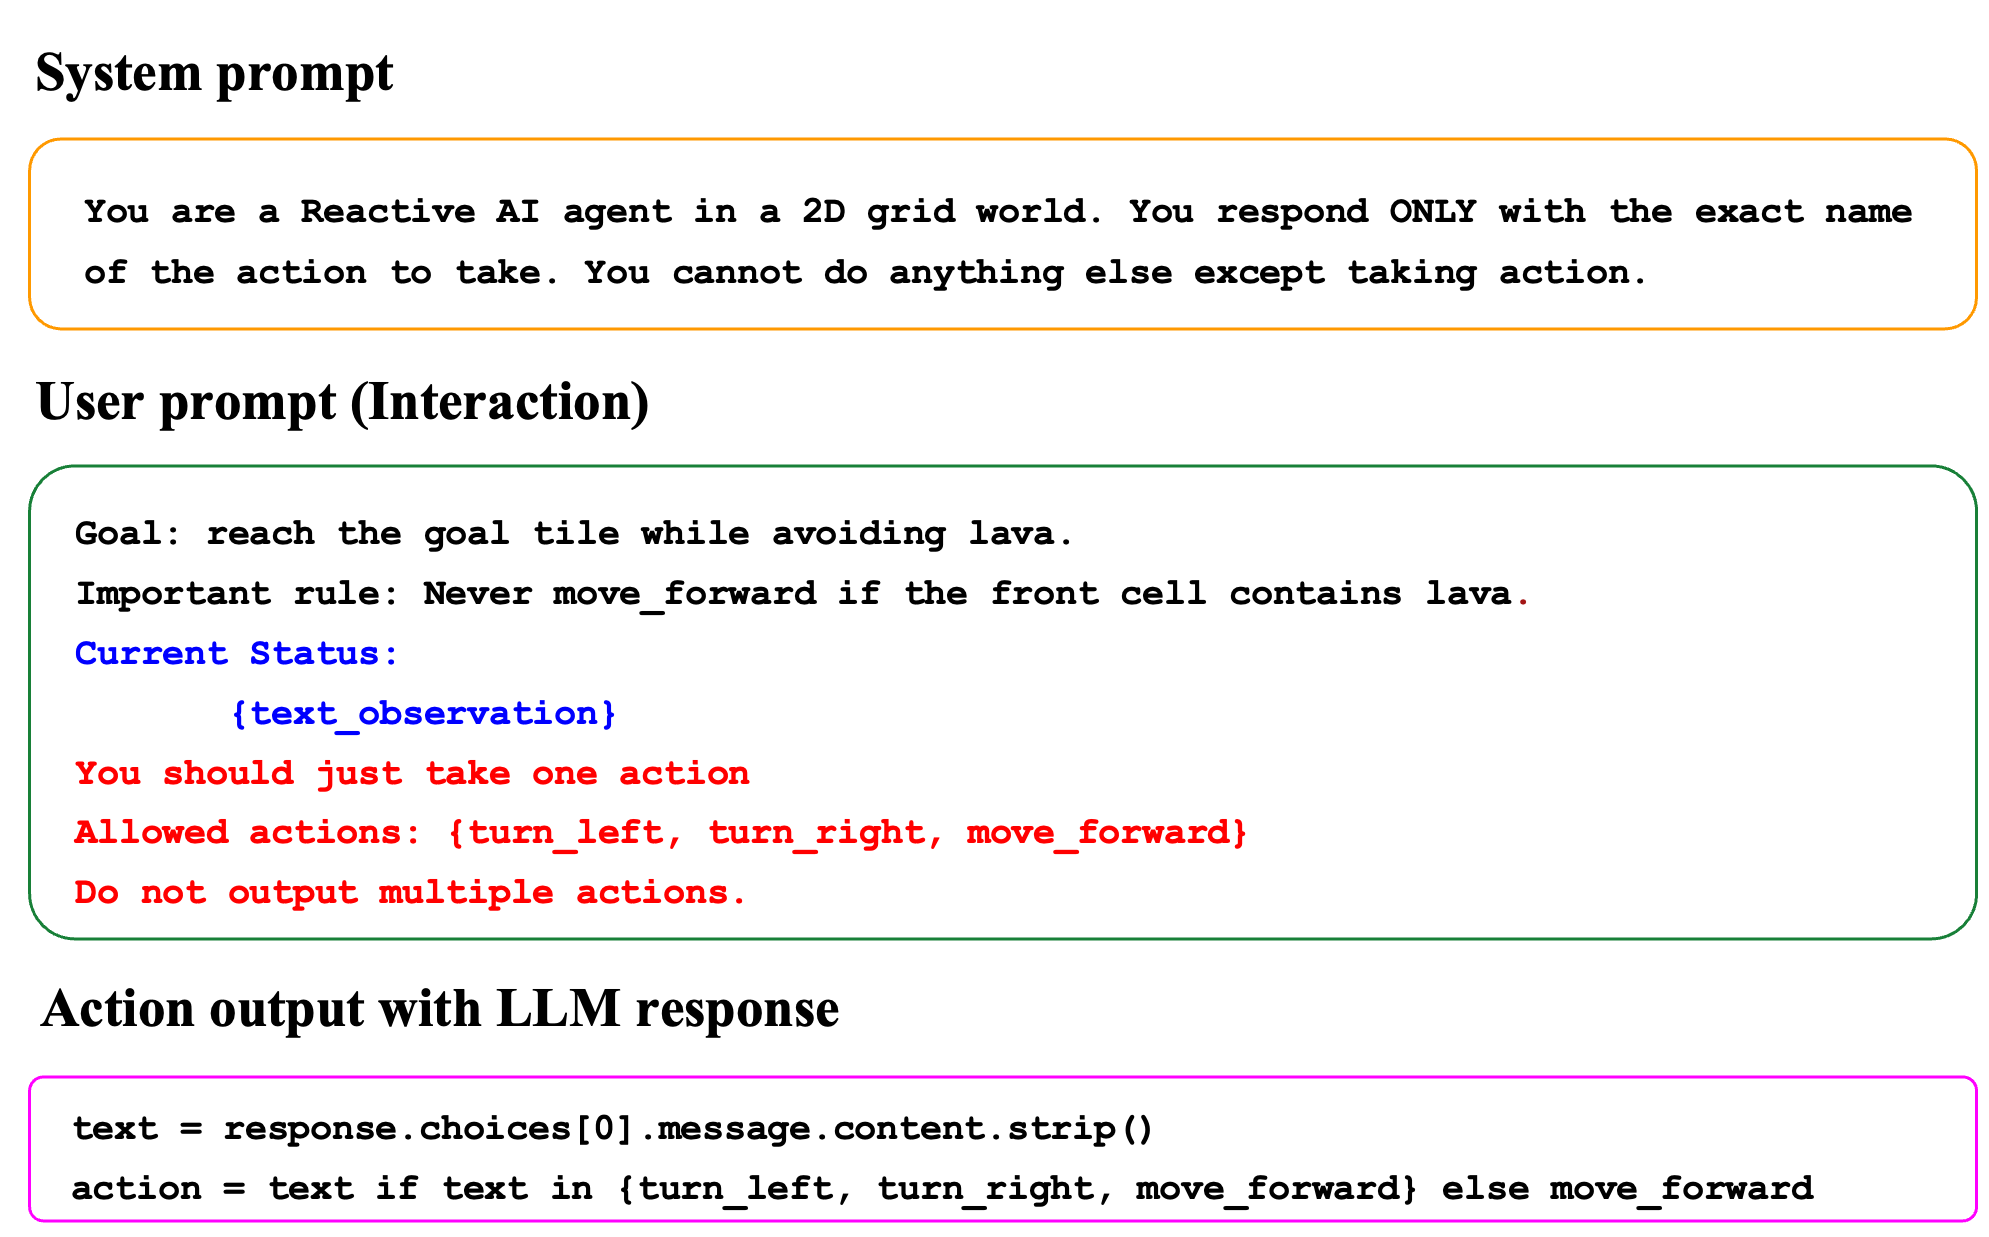
\includegraphics[width=0.8\linewidth]{Figures/Reactive.png}
    \caption{Prompt of reactive agent}
    \label{fig:reactive}
\end{figure}

The text observation should consider the ego agent state (i.e., the position and direction), neighbors box states, the goal and lava position. A example of text observation is as follows:
\begin{figure}
    \centering
    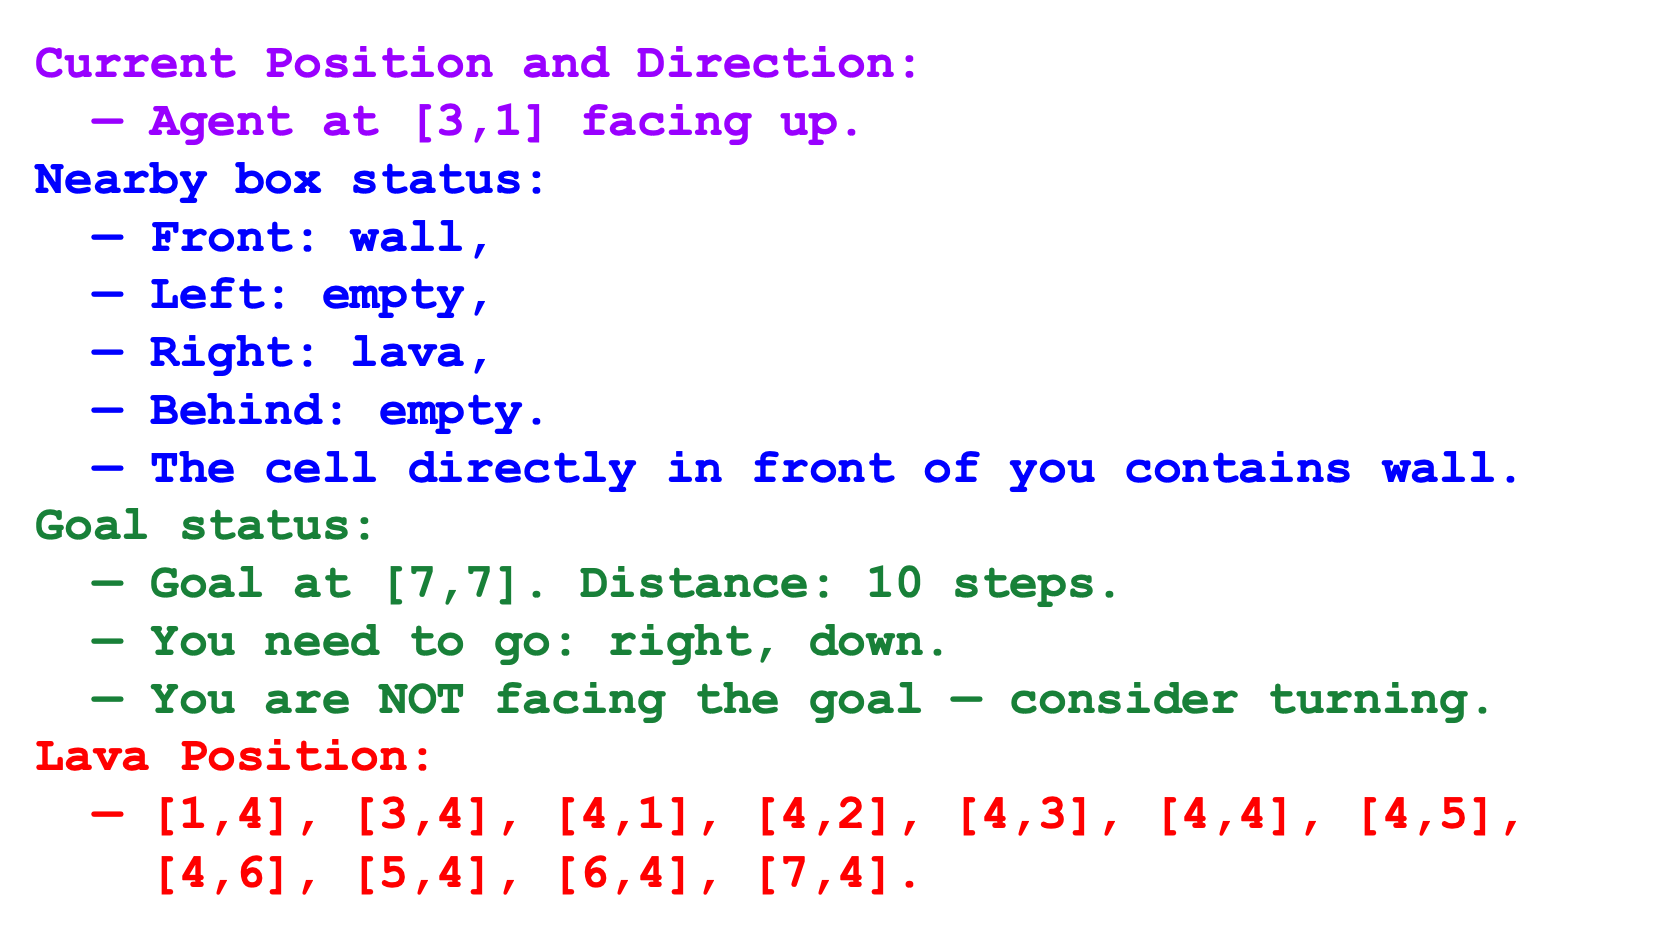
\includegraphics[width=0.9\linewidth]{Figures/State.png}
    \caption{An example of the text observation}
    \label{fig:state}
\end{figure}
\subsection{Chain of Thought}
Chain of Thought (CoT)~\citep{wei2023chainofthoughtpromptingelicitsreasoning} is a simple but effective prompt engineering technique that instructs the model to output step-by-step reasoning before deciding upon its action. For our implementation  of CoT, we instruct the model to "\texttt{Output a careful step-by-step analysis of what the rules are, what has happened in the past states and actions, what actions are valid, and what would be the best strategy to take.}" In our tests, this leads to outputs that first analyze the current position/orientation, goal direction, candidate actions, and overall strategy before deciding upon an action.
% \begin{figure}[htbp]
%     \centering
%     
\includegraphics[width=0.8\linewidth]{Figures/CoT.png}
%     \caption{The impact of Chain of Thought prompting.}
%     \label{fig:CoT}
% \end{figure}
\subsection{ReAct}

ReAct (Reason + Act)~\citep{yao2023react} integrates reasoning and action generation within a single interaction loop. Instead of directly predicting an action from the observation, the model first produces a short reasoning step describing its interpretation of the environment state, followed by the selected action. This intermediate reasoning encourages the model to analyze the current situation before deciding on the next move. Each step therefore follows the structure \textit{Thought $\rightarrow$ Action}, where the Thought explains the reasoning and the Action specifies the navigation command.

In our implementation, the MiniGrid environment state is converted into a structured textual observation describing the agent's position, orientation, nearby tiles, and goal direction. This observation, together with environment rules and recent reasoning history, is included in the prompt provided to the LLM. The model then outputs a Thought--Action pair, from which the action (\texttt{turn\_left}, \texttt{turn\_right}, or \texttt{move\_forward}) is extracted and executed in the environment. The resulting observation is appended to the prompt history and the interaction continues until the goal is reached or the episode terminates.
\subsection{Tree of Thought}

Unlike single-path reasoning strategies such as Chain-of-Thought\cite{yang2024buffer}, the Tree-of-Thought (ToT) agent~\cite{yao2023tree} explores multiple candidate actions at each timestep and selects the most promising one through explicit evaluation and pruning. At each step, the agent enumerates all available actions (e.g., \texttt{turn\_left}, \texttt{turn\_right}, \texttt{move\_forward}) and treats each as a branch in a shallow reasoning tree. For every candidate, the LLM is prompted to imagine the resulting state, estimating the new agent position, orientation, and surrounding tile layout based solely on the current observation and the proposed action.

Each imagined successor state is then evaluated by the LLM, which scores branches based on estimated goal proximity, perceived hazards such as lava tiles and walls, and overall progress toward task completion. Branches deemed unsafe or unproductive are pruned, and the agent executes the highest-scoring action in the environment. The resulting observation is fed back into the next iteration of the loop. Because both imagination and evaluation are handled entirely by the LLM, the ToT agent operates as a depth-2 lookahead search driven by language-based reasoning.

\subsection{Buffer of Thought}
Buffer of Thought (BoT) augments action selection with a compact strategy memory rather than full multi-branch search like Tree-of-Thought \cite{yao2023tree}. Following the idea of reusable thought templates proposed by Yang et al. \cite{yang2024buffer}, our implementation maintains a small meta-buffer of navigation templates (e.g., direct navigation, obstacle avoidance, lava crossing, and recovery). At each timestep, the observation is first distilled into structured features (agent position, orientation, nearby occupancy, goal direction, and hazards). The meta-buffer then retrieves the most suitable template based on the current context, including whether the agent is blocked, in a repeated state, or likely to reduce goal distance by moving forward.

Conditioned on the selected template, the agent forms a ranked list of candidate actions and prompts the LLM to choose one action from this restricted set. A hard safety rule is applied afterward: if the front cell is unsafe (wall or lava), \texttt{move\_forward} is overridden by a safe turning action. This design keeps per-step reasoning lightweight while preserving context-sensitive behavior.

In addition, BoT includes post-episode adaptation. When an episode fails, we classify a failure signature (e.g., lava death, timeout, or looping) together with a coarse grid category. If the same signature repeats, the agent asks the LLM to synthesize a one-sentence strategy template from recent trajectory traces and adds it to the meta-buffer under deduplication and capacity limits. Compared with Tree-of-Thought-style explicit branching, this template-retrieval mechanism is cheaper at inference time when the seed templates are well crafted and relevant. If the agent has not explored enough or has not yet accumulated useful templates, performance can be weaker until more effective templates are built over time \cite{yang2024buffer}.

% \subsection{LLM agent for navigation}
% \subsection{LLM agents}
